\documentclass{beamer}
\usetheme{metropolis}

\usepackage{amsmath, amssymb, amsthm}
\usepackage{cite, graphicx, latexcolors}
\usepackage{ragged2e, microtype}
\usepackage{url, parskip, hyperref}
\usepackage{array, tikz, flowchart}
\usepackage[dvipsnames]{xcolor}

\hypersetup{colorlinks=true,}
\setbeamercolor{title}{fg=orange}

\usetikzlibrary{arrows.meta, calc, chains, quotes, positioning, shapes.geometric}
\tikzset{FlowChart/.style={
    node distance = 5mm and 10mm,
    start chain = A going right,
    base/.style = {draw, minimum width=16mm, minimum height=19mm, align=center, on chain=A, text width=4cm},
    process/.style = {base},
    rounded/.style = {base, rounded corners},
    every edge quotes/.style = {auto=right}
}}

\title[NMPC Implementation]{
    \textbf{Implementation of Nonlinear MPC \\
    with Stoch 4 or Biped robot
\subtitle[Presentation]{\textcolor{brown}{
    \textbf{FoR Project Presentation - 1} \\
}}}}
\author[BRAMA]{%
Team-5 BRAMA \quad \scriptsize \\
\begin{tabular}{lllll}
    Biswadeep &
    Rithwik &
    Akhil &
    Moin &
    Ashrith
\end{tabular}
\vspace{2em}
}
\institute[IISc]{    
    Robert Bosch Centre for Cyber Physical Systems,\\
    Indian Institute of Science
}
\date{\scriptsize\today}
\begin{figure}
    
\includegraphics[width=0.25\linewidth]{Common/rbccps.png}
\end{figure}


\begin{document}


% \section*{Titlepage}
\begin{frame}\titlepage\end{frame}\normalfont


% \section*{Outline}
\begin{frame}{Outline}
	\begin{enumerate}
		\item Introduction
		\item Literature Survey
		\item Motivation
		\item Implementation strategy
		\item Project Timeline
	\end{enumerate}
\end{frame}\normalfont


% \section{Introduction}
\begin{frame}{Introduction}
        \setlength{\itemsep}{1em}
	\setlength{\parskip}{2pt}
	\begin{itemize}\small
            \item Legged animals have shown their versatile mobility to traverse challenging terrains via a well-coordinated dynamic motions.
                \begin{itemize}\scriptsize
                    \item Design and control remains a difficult problem
                \end{itemize}
		\item \textbf{Model Predictive Control (MPC)}
                \begin{itemize}\scriptsize
                    \item A method that predicts a system's future behavior and calculates optimal control action to follow a desired path.
                    \item Uses a Receding Horizon Approach
                    \item Real-time execution of MPC controller is a challenge for high degree-of-freedom systems
                \end{itemize}
	\end{itemize}
\end{frame}\normalfont


\begin{frame}{Literature Survey}
        \scriptsize{Key paper that will be implemented:}

	\scriptsize
	\centering
	\begin{table}[ht]
		\resizebox{\textwidth}{!}{
			\begin{tabular}{|>{\centering\arraybackslash}p{2.5cm}|>{\centering\arraybackslash}p{3.0cm}|>{\centering\arraybackslash}p{3.5cm}|>{\centering\arraybackslash}p{5.0cm}|}
				\hline
				\textbf{Title} & \textbf{Authors} & \textbf{Objectives} & \textbf{Key Takeaways} \\
				\hline
				Real-time Model Predictive Control for Versatile Dynamic Motions in
				Quadrupedal Robots                
                    &    Yanran Ding, Abhishek Pandala, and Hae-Won Park 
                    & 
                        This paper presents a new Model Predictive
				Control (MPC) framework for controlling various dynamic
				movements of a quadrupedal robot. 
                    &
                    \begin{itemize}
                        \item New NMPC framework without parametrisations
                        \item Variation-based linearization used
                        \item Vectorization algorithm laid out
                    \end{itemize}
                    \\
				\hline
			\end{tabular}
		}
	\end{table}
\end{frame}

\begin{frame}{Literature Survey}
	\scriptsize
	\centering
	\begin{table}[ht]
		\resizebox{\textwidth}{!}{
			\begin{tabular}{|>{\centering\arraybackslash}p{2.5cm}|>{\centering\arraybackslash}p{3.0cm}|>{\centering\arraybackslash}p{3.5cm}|>{\centering\arraybackslash}p{5.0cm}|}
				\hline
				\textbf{Title}                    & \textbf{Authors}                                & \textbf{Objectives}                                                                                                                                                                                        & \textbf{Key Takeaways}                                                                                           \\
				\hline
				Online Planning for Autonomous Running Jumps Over Obstacles in High-Speed Quadrupeds & Hae-Won Park, Patrick M. Wensing, and Sangbae Kim 
				& Presents a novel control framework for quadrupedal robots, enabling dynamic running jumps over obstacles through model predictive control and constrained nonlinear optimization. & Introduces a model predictive control (MPC) framework for dynamic jumping in quadrupeds.                                                                                                                                                                                                                                      \\
				\hline
				Successive Linearization NMPC for a Class of
				Stochastic Nonlinear Systems      & Mark Cannon, Desmond Ng, and Basil Kouvaritakis & Presents a receding horizon control methodology for systems
with nonlinear dynamics, additive stochastic uncertainty                                                                                                                         & Can be referred for successive linearization for operating points                                                                     \\
				\hline
				Variation-Based Linearization of Nonlinear
				Systems Evolving on SO(3) and S^2 & Guofam Wu and Koushil Sreenath                  & Propose a variation-based method to linearize the nonlinear dynamics of robotic systems, whose configuration spaces contain the manifolds S2 and SO(3), along dynamically feasible reference trajectories. & A variation-based method to linearize a nonlinear system, whose dynamics evolve on complex manifolds that contain SO(3) and S2 , along a desired reference trajectory. \\
				\hline
			\end{tabular}
		}
	\end{table}
\end{frame}



\begin{frame}{Motivation / Objective}
        For the key paper

	\begin{enumerate}
		\item Linearize single RBD rotations matrices \textbf{without resorting to parametrization}
		\item Avoid issues arising from using \textbf{local coordinates}\\
		      \textit{Euler angles:} Have singularity issues; Gimbal lock\\
		      \textit{Quaternions:} Unwinding issues
		\item Enable a \textit{QP formulation} for \textbf{real-time execution} using a linearization  technique and use of \textit{configuration error function} on $SO(3)$
		\item Development of a \textbf{singularity-free MPC formulation} with consistent performance even when executing motions that involve complex 3D rotations
	\end{enumerate}
\end{frame}


\begin{frame}{Overview}
	\resizebox{\textwidth}{!}{%
    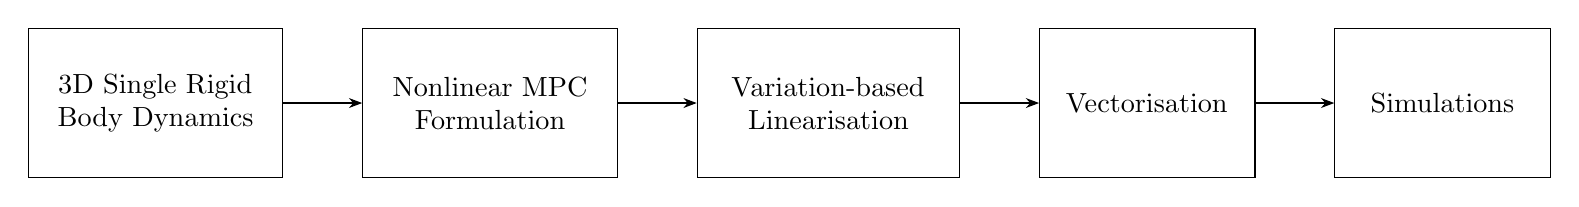
\begin{tikzpicture}[FlowChart]
        \node [process, text width=3cm] {
            3D Single Rigid Body Dynamics
        };
        \node [process, text width=3cm] {
            Nonlinear MPC Formulation
        };
        \node [process, text width=3.1cm] {
            Variation-based Linearisation
        };
        \node [process, text width=2.5cm] {
            Vectorisation
        };
        \node [process, text width=2.5cm] {
            Simulations
        };
    
        \draw [arrows=-Stealth]
        (A-1) edge (A-2)
        (A-2) edge (A-3)
        (A-3) edge (A-4)
        (A-4) edge (A-5);
    \end{tikzpicture}
}


	\setlength{\itemsep}{1em}
	\setlength{\parskip}{2pt}
	\begin{enumerate}\small
		\item Template model
		      \begin{enumerate}\scriptsize
		      	\item 3D Single Rigid Body Dynamics
		      	\item Global coordinate frame for rotations
		      \end{enumerate}
		\item Nonlinear MPC formulation
		      \begin{enumerate}\scriptsize
		      	\item Non-linear terms for rotations in state space model
		      	\item Formulate the NMPC as a constrained optimisation problem
		      \end{enumerate}
		\item Variation-based Linearisation
		      \begin{enumerate}\scriptsize
		      	\item Succesive Linearisation
		      \end{enumerate}
		\item Vectorisation
		      \begin{enumerate}\scriptsize
		      	\item Using Kronecker products
		      \end{enumerate}
		\item Simulations
		      \begin{enumerate}\scriptsize
		      	\item Different walking styles
		      \end{enumerate}
	\end{enumerate}
\end{frame}


\begin{frame}{Implementation Strategy}
    \setlength{\itemsep}{1em}
    \setlength{\parskip}{2pt}
    \begin{enumerate}\small
        \item Prototype the functions: Two main modules
            \begin{enumerate}\scriptsize
                \item \textbf{RBD class} with parameters \texttt{rbdmodel(x, u)}
                \item \textbf{NMPC class} with an objective function
                \begin{enumerate}\scriptsize
                    \item Vectorise method \texttt{.vectorise()}
                    \item QPSolve method \texttt{.qpsolve()}, using a library for solving QP
                \end{enumerate}
            \end{enumerate}
        \item Validate using an initial Simulation setup
            \begin{enumerate}\scriptsize
                \item On Gazebo
            \end{enumerate}
        \item Deliverable: \texttt{pyNMPC}\\
            \begin{enumerate}\scriptsize
                \item A library that has all the functionality described above
            \end{enumerate}
        \item (*) Library-free implementation
            \begin{enumerate}\scriptsize
                \item Custom QP solver, as mentioned in the paper
                \item Exploits the sparsity structure of the KKT matrix
            \end{enumerate}
        \item (*) Implement the vectorisation parts in C++
    \end{enumerate}

\end{frame}


\begin{frame}{Project Timeline}
	\scriptsize
\centering
\begin{table}[ht]
    \resizebox{\textwidth}{!}{
        \begin{tabular}{|>{\centering\arraybackslash}p{1.2cm}|>{\centering\arraybackslash}p{3.5cm}|>{\centering\arraybackslash}p{5.5cm}|}
            \hline
            \textbf{Week} & \textbf{Objective}                                  & \textbf{Key Deliverables}                                                  \\
            \hline
            \textbf{1}    & \textbf{Initial Research}& Literature review,  Understanding the model\\
            \hline
            \textbf{2}    & \textbf{Preliminary Model Implementation}& Implementation in Python \\
            \hline
            \textbf{3}    & \textbf{Final Model Implementation}& Implementation in C++ (With a Python interface)\\
            \hline
            \textbf{4}    & \textbf{Simulation}& Simulation in Gazebo\\
            \hline
            \textbf{5}    & \textbf{Testing and Validation}& Validation of our implementation using Gazebo simulation for different walking styles\\
            \hline
            \textbf{6}    & \textbf{Report}& Preparation of Report and additional objectives (if any)\\
            \hline
            \textbf{7}    & \textbf{Final Presentation}& Final report, presentation slides, demo videos                             \\
            \hline
        \end{tabular}
    }
\end{table}

\end{frame}


\begin{frame}
	\LARGE{Thank You!}
\end{frame}\normalfont


\begin{frame}{RBD model}
\begin{figure}
    \centering
    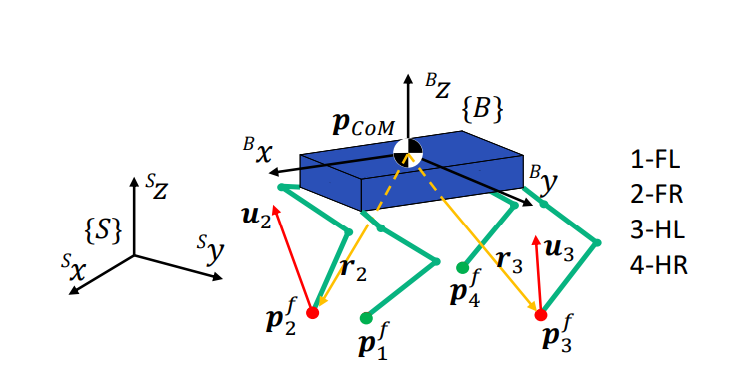
\includegraphics[width=0.6\linewidth]{Illustration-RBD-model.png}
    \caption{Illustration of the 3D Single RBD model}
    \label{fig:rbd-model}
\end{figure}
\begin{equation*}
    \mathbf{\dot{x}} = f(\mathbf{x}, \mathbf{u}) = 
    \begin{bmatrix}
    \mathbf{\dot{p}} \\
    \mathbf{\ddot{p}} \\
    \mathbf{\dot{R}} \\
    \boldsymbol{\dot{\omega}}
    \end{bmatrix}
    =
    \begin{bmatrix}
    \mathbf{\dot{p}} \\
    \frac{1}{M} \mathbf{f} - \mathbf{a_g} \\
    \mathbf{R} \cdot \hat{\boldsymbol{\omega}} \\
    {}^{B} \mathbf{I}^{-1}(R^T \boldsymbol{\tau} - \hat{\boldsymbol{\omega}} {}^{B} \mathbf{I} \boldsymbol{\omega})
    \end{bmatrix}
\end{equation*}
\end{frame}


\begin{frame}{Non-Linear MPC formulation}

\begin{equation*}
\begin{aligned}
    & \text{minimize} \quad \sum_{k=1}^{N-1} \ell(x_k, u_k) + \ell_T(x_N) \\
    & \text{subject to} \quad x_{k+1} = g(x_k, u_k), \quad x_1 = x_\text{op}, \\
    & x_k \in \mathcal{X}, \quad k = 1, 2, \dots, N, \\
    & u_k \in \mathcal{U}, \quad k = 1, 2, \dots, N-1
\end{aligned}
\end{equation*}

\begin{itemize}
    \item Stage cost
    \item Terminal cost
\end{itemize}

\end{frame}


\begin{frame}{Resources}

\begin{itemize}
    \item \url{https://github.com/YanranDing/RF-MPC}
        \begin{itemize}
            \item The author's subsequent work
            \item They implement some of the functions in MATLAB
        \end{itemize}    
\end{itemize}

\end{frame}


\end{document}
